% Worked example of one auction (analyze/auction_schematic.py).
\begin{figure}[H]
    \centering
    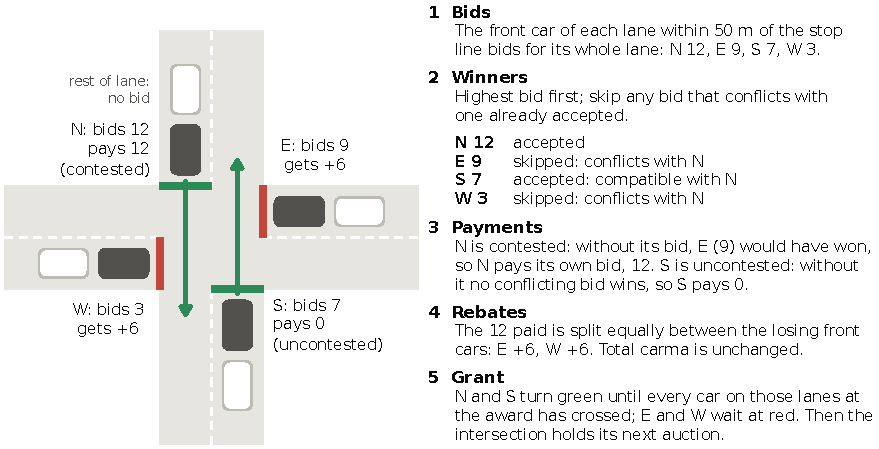
\includegraphics[width=\linewidth]{auction_schematic.pdf}
    \caption{One auction at a four-way intersection, assuming each lane only goes straight, so
    north (N) and south (S) are compatible and both conflict with east (E) and west (W). Only the
    front car of each lane bids (eq.~\eqref{eq:bid}); the greedy rule accepts N, then S
    (eq.~\eqref{eq:greedy}); N pays its bid because it displaced E, S rides free
    (eq.~\eqref{eq:payment}); and the losers share the payment (eq.~\eqref{eq:rebate}). Stop
    lines show the signal after the auction: green for N and S, red for E and W.}
    \label{fig:auction_schematic}
\end{figure}
